\documentclass[12pt]{article}
\usepackage{graphicx} % Required for inserting images
\usepackage{hyperref} % Required for adding clickable links

\title{Annotated Bibliography of Current Research}
\author{Tahira Tariq}
\date{September 2024 - November 2024}

\begin{document}
\maketitle

\section{The Mirror-Neuron System and the\\Consequences of its Dysfunction}
\textit{Authors: Marco Iacoboni, Mirella Dapretto}\\
This paper delves into the mirror neuron system, particularly how it helps humans understand the actions and intentions of others, which is crucial for interpreting nonverbal cues like body language and facial expressions. It also explores the potential dysfunction of this system in conditions like autism, affecting nonverbal communication.\\

\noindent Iacoboni, M., \& Dapretto, M. (2006). The mirror neuron system and the\\consequences of its dysfunction.\textit{Nature Reviews. Neuroscience},\\\textit{7}(12), 942–951. \href{https://doi.org/10.1038/nrn2024}{doi.org/10.1038/nrn2024}.\\

\noindent macaque:\\
\begin{figure}[ht]
    \centering
    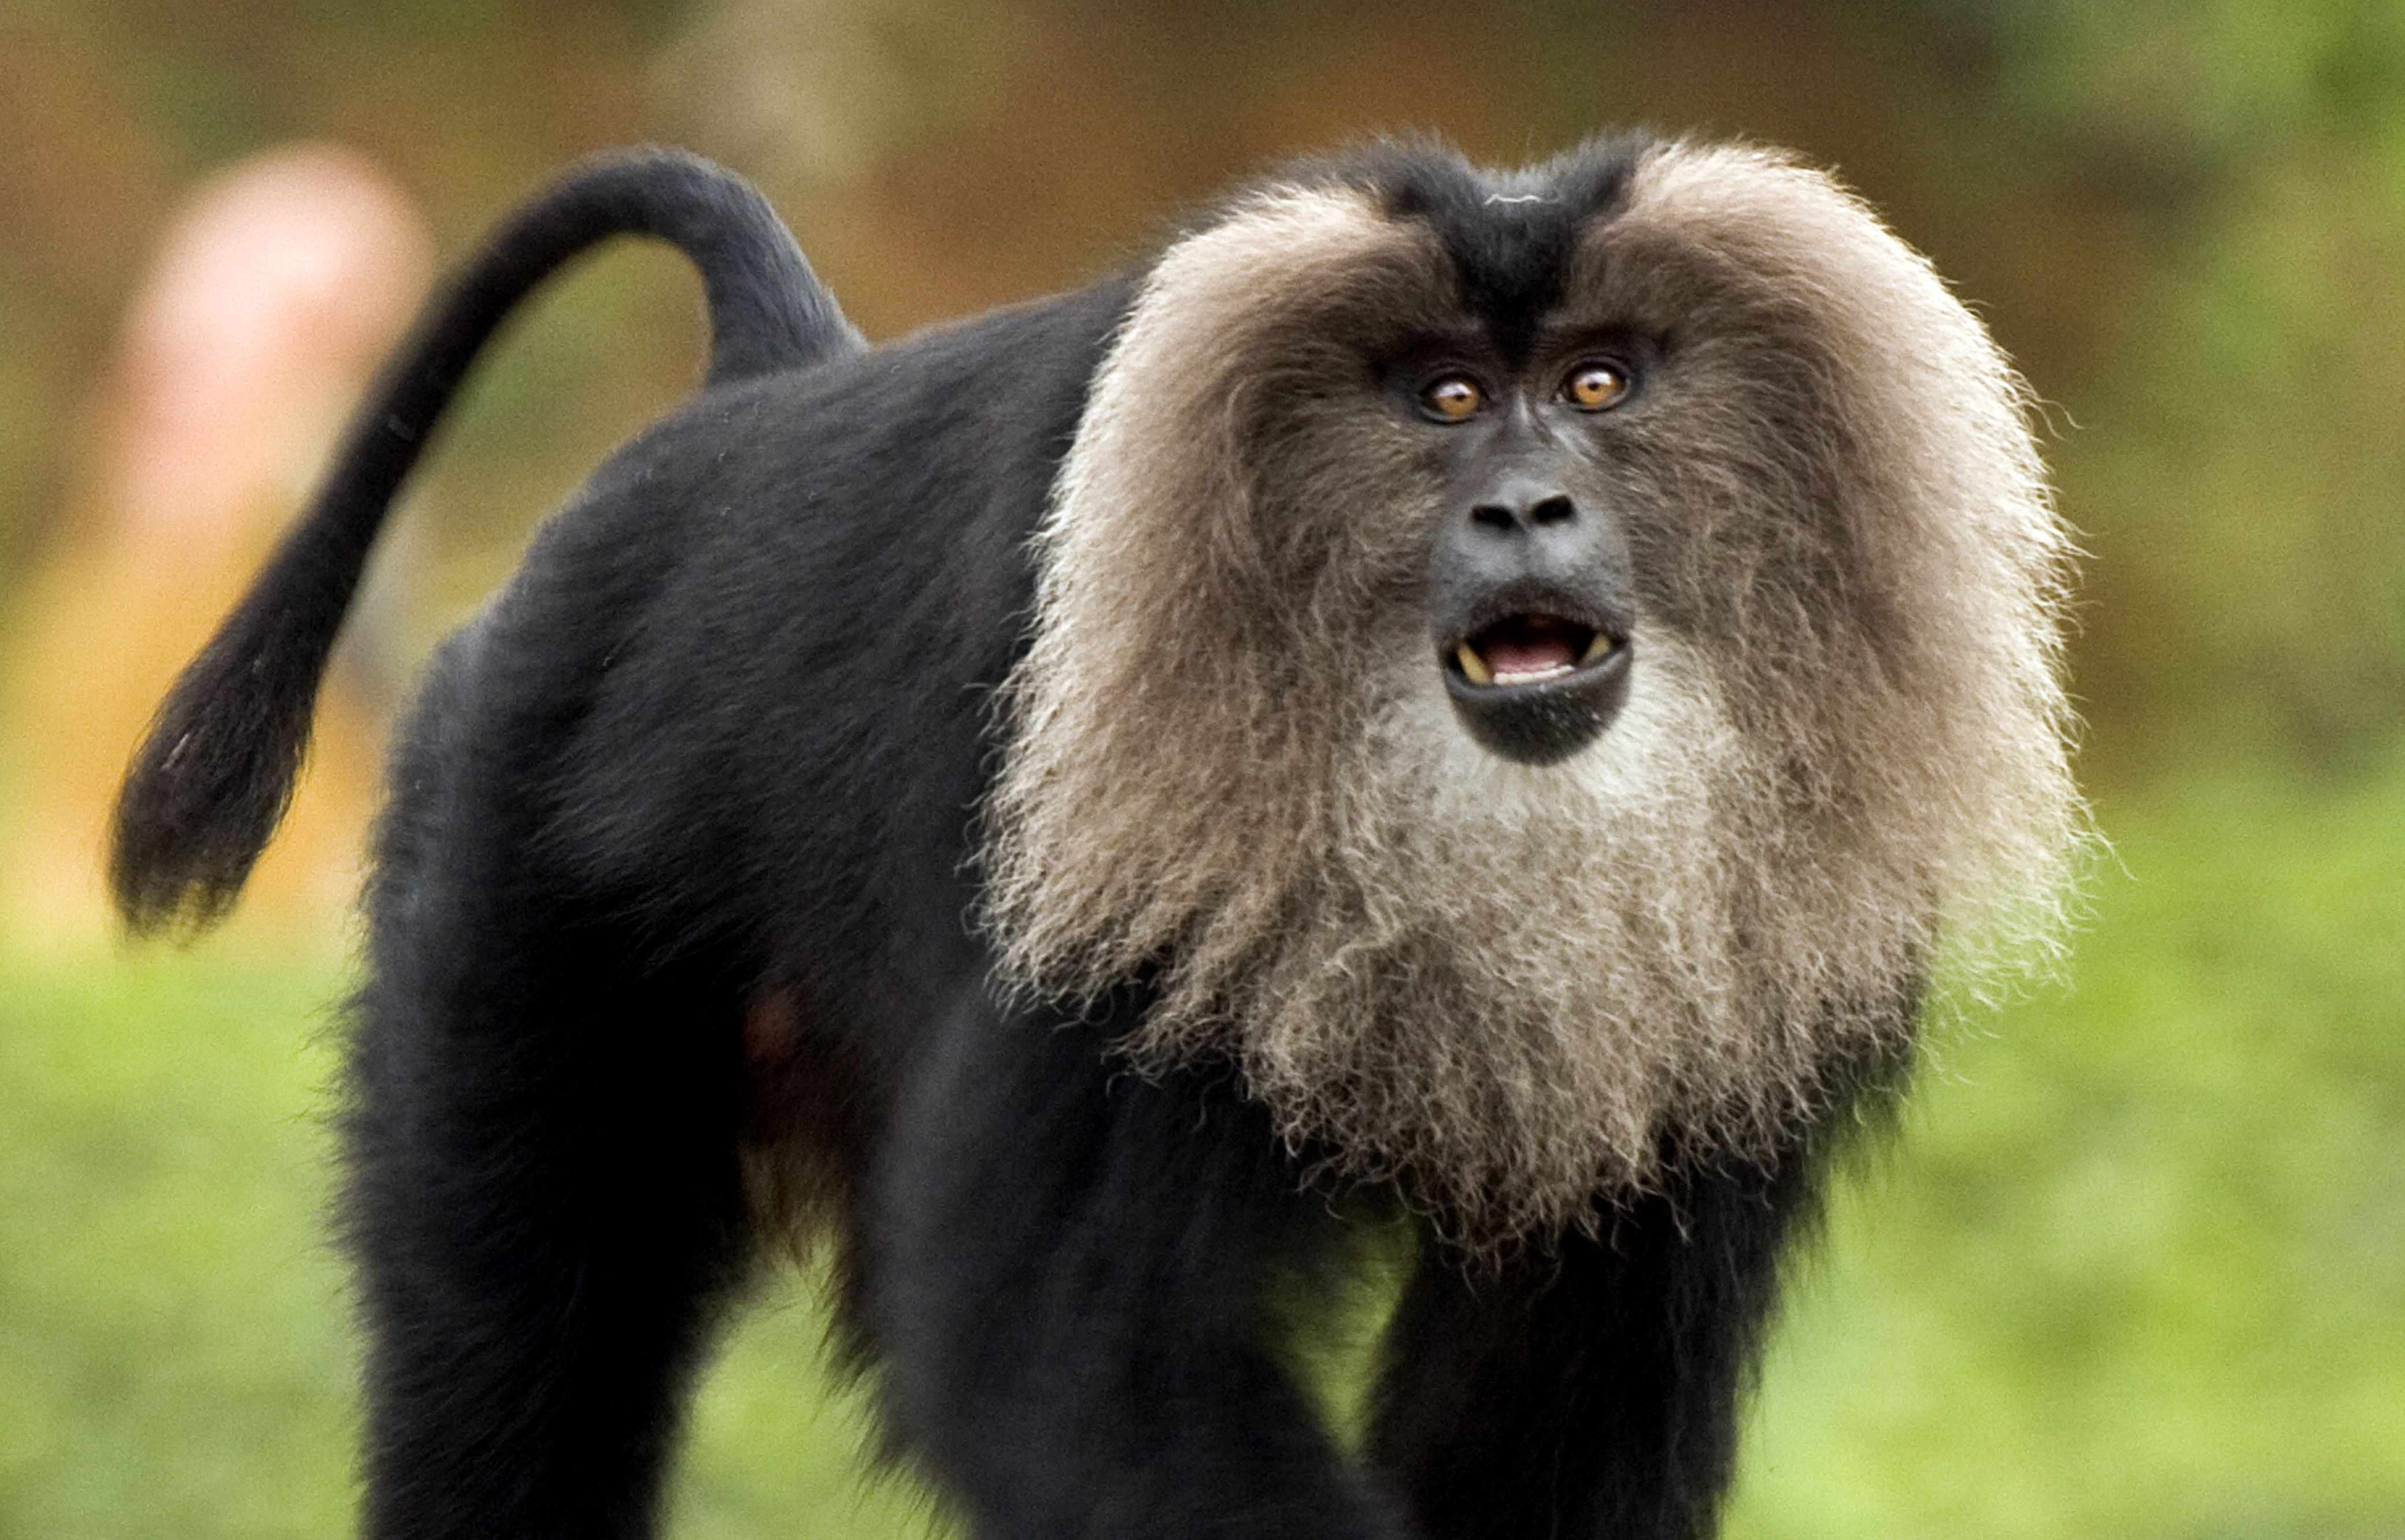
\includegraphics[width=0.5\textwidth]{macaque.jpg} %
    \caption{Lion-tailed macaque. Image source: \href{https://commons.wikimedia.org/wiki/File:Lion-tailed_macaque_by_N_A_Nazeer.jpg}{Wikimedia Commons}}
    \label{fig:macaque}
\end{figure}

\noindent premotor and posterior parietal cortex (of the macaque brain) but these are human brains:\\
\begin{figure}[ht]
    \centering
    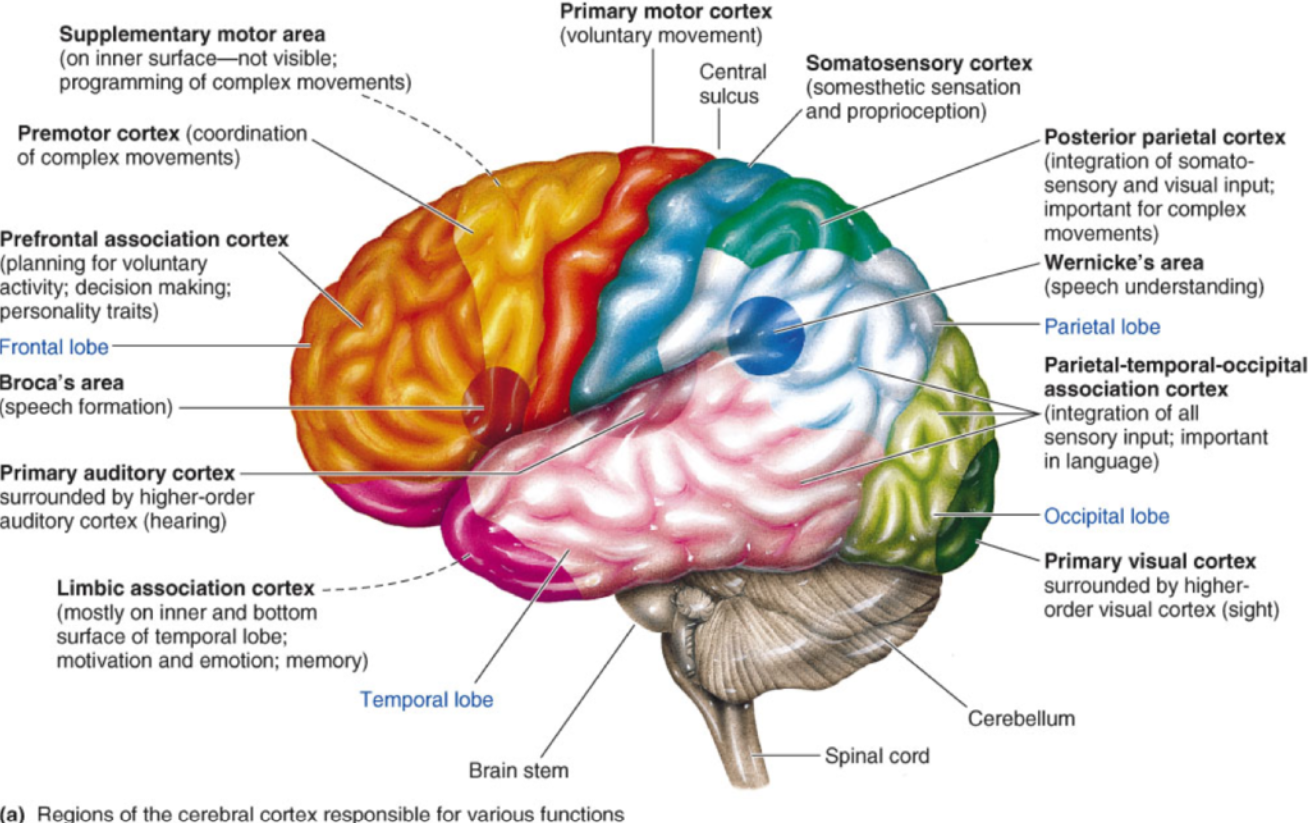
\includegraphics[width=0.5\textwidth]{brain1.png} %
    \caption{Premotor cortex. Image source: \href{https://o.quizlet.com/il-zAgEMk31L--6ugy5MGw_b.png}{Quizlet}}
    \label{fig:pre}
\end{figure}

\begin{figure}[ht]
    \centering
    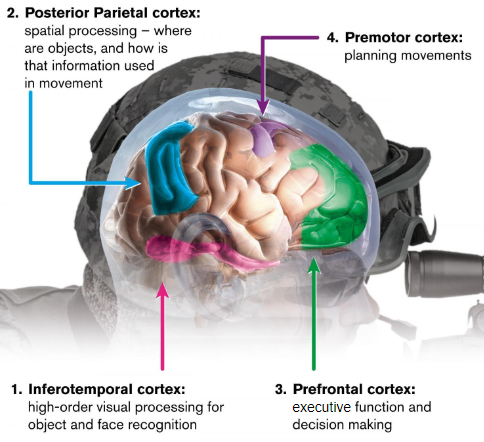
\includegraphics[width=0.5\textwidth]{brain2.png} %
    \caption{Posterior parietal cortex. Image source: \href{https://www.braininitiative.org/wp-content/uploads/2017/08/Posterior-Parietal-Cortex-170726.jpg}{Brain Initiative Alliance}}
    \label{fig:post}
\end{figure}

\noindent in humans: mirror neuron areas are located in the posterior\\inferior frontal gyrus and adjacent ventral premotor cortex, and in the\\rostral part of the inferior parietal lobule.\\

\noindent in macaques: mirror neurons located in area F5 in the inferior frontal cortex and area PF/PFG in the inferior parietal cortex.\\

\noindent sensorimotor integration: complex process in the central nervous system where sensory information from multiple sources is selectively and\\rapidly integrated to produce task-specific motor output.\\

\noindent mirror neurons in monkeys respond to the sound of actions and\\code the intention associated with the observed action.

vs

\noindent mirror neuron system in humans is related to imitation +\\use of limbic system.\\

limbic system:

\begin{itemize}
    \item processes and regulates emotion and memory while also dealing with sexual stimulation and learning.
    \item behavior, motivation, long-term memory, and sense of smell\\is also related.
\end{itemize}

\noindent Evidence of MNS abnormalities in autism spectrum disorder (ASD)\\is provided by structural MRI, magnetoencephalography,\\ electroencephalography, transcranial magnetic stimulation and functional MRI (fMRI). fMRI data show that children with ASD have reduced MNS activity during social mirroring and that MNS activity correlates with the severity of disease: the higher the impairment, the lower the MNS activity in ASD.\\

\noindent MRI: a medical imaging technique that provides precise details of your body parts, especially organs and soft tissues, with the help of magnetic fields and radio waves.\\

\noindent Magnetoencephalography (MEG): a functional neuroimaging technique for mapping brain activity and locating seizures by recording magnetic fields produced by electrical currents occurring naturally in the brain, using very sensitive magnetometers.\\

\noindent Electroencephalography (EEG): a test to monitor the electric sensitivity of the brain by recording an electrogram of the spontaneous electrical activity of the brain and thereby detect disorders if any, using electrodes.\\

\noindent Transcranial Magnetic Stimulation (TMS): a noninvasive form of brain stimulation in which a changing magnetic field is used to induce an electric current at a specific area of the brain through electromagnetic induction.\\

\noindent fMRI: measures brain activity by detecting changes associated with blood flow.

\section{The Role of Beta-Frequency\\Neural Oscillations in Motor Control}
\textit{Authors: Nick J. Davis, Simon P. Tomlinson and Helen M. Morgan}\\
This study discusses how beta oscillations (15-30 Hz) are linked to\\motor control, particularly how they change during voluntary movement and return to baseline after movement. It explores the hypothesis that\\beta activity represents the status quo and how its disruption is associated with motor disorders like Parkinson’s disease. The paper also examines\\the use of transcranial alternating current stimulation (tACS) to investigate the role of these oscillations in motor control.\\


\noindent Davis, Nick J, et al. “The Role of Beta-Frequency Neural Oscillations in Motor Control.” Journal of Neuroscience, vol. 32, no. 2, 11 Jan. 2012, pp. 403–404, \href{https://doi.org/10.1523/jneurosci.5106-11.2012}{doi.org/10.1523/jneurosci.5106-11.2012}.\\

\begin{figure}[ht]
    \centering
    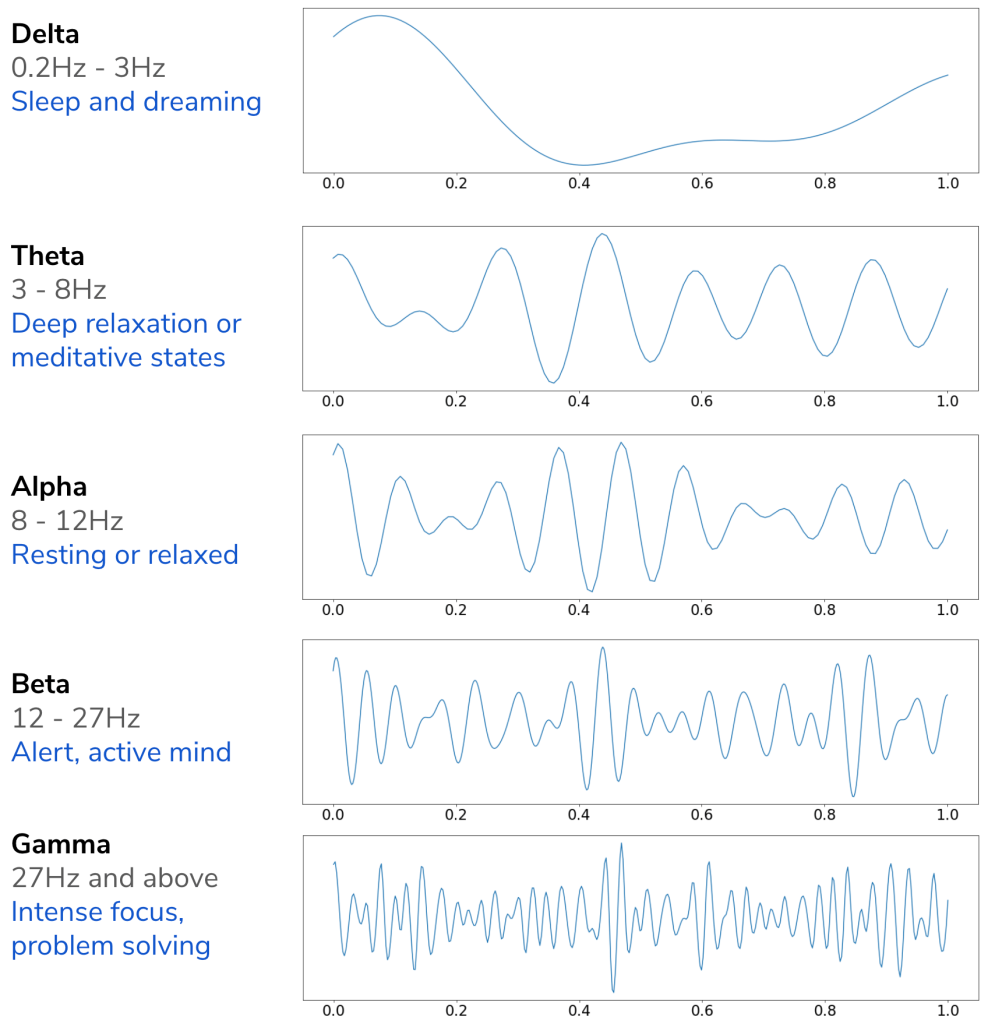
\includegraphics[width=0.5\textwidth]{brain_waves.png} %
    \caption{Basics of neural oscillations. Image source: \href{https://d2z0k1elb7rxgj.cloudfront.net/uploads/2022/09/brain-waves-988x1024.png}{EMOTIV}}
    \label{fig:waves}
\end{figure}

\section{Gamma-Band Synchronization in the\\Macaque Hippocampus and Memory Formation}

\noindent\textit{Authors: Michael J. Jutras, Pascal Fries and Elizabeth A. Buffalo}\\

\noindent This paper focuses on gamma-band synchronization (30-100 Hz)\\in the hippocampus and its role in memory formation. It provides evidence that gamma synchronization during the encoding phase of a memory task\\predicts better subsequent recognition memory. The study highlights\\the importance of precise timing in neuronal activity for long-term\\synaptic changes, which are crucial for memory encoding.\\

Jutras, Michael J, et al. “Gamma-Band Synchronization in the\\Macaque Hippocampus and Memory Formation.” Journal of Neuroscience, vol. 29, no. 40, 7 Oct. 2009, pp. 12521–12531, www.jneurosci.org/content/29/40/12521, \href{https://doi.org/10.1523/jneurosci.0640-09.2009}{doi.org/10.1523/jneurosci.0640-09.2009}\\

\noindent tACS - transcranial alternating current stimulation:

\begin{itemize}
    \item a form of non-invasive brain stimulation
    \item sinusoidal alternating electric currents are delivered to the scalp\\to affect mostly cortical neuron
    \item supposed to modulate brain function and, in turn, cognitive processes by entraining brain oscillations + inducing long-term synaptic plasticity
\end{itemize}

\section{Imaging Functional Neuroplasticity in\\Human White Matter Tracts}
\noindent\textit{Authors: Cathy J. Price, Karl J. Friston}\\

\noindent This paper reviews the use of MRI, particularly diffusion tensor imaging (DTI), to study neuroplasticity in white matter tracts. It discusses how motor training can lead to structural and functional changes in white matter, such as the internal capsule and corpus callosum.\href{https://www.frontiersin.org/journals/neuroscience/articles/10.3389/fnins.2024.1441002/full}{The study also explores how these changes are associated with improved motor performance and the underlying mechanisms of neuroplasticity, including myelination and axonal transmission efficiency}.\\

\noindent Frizzell, T.O., Phull, E., Khan, M. \textit{et al.} Imaging functional neuroplasticity in human white matter tracts.\textit{Brain Struct Funct} \textbf{227}, 381–392 (2022). \href{https://doi.org/10.1007/s00429-021-02407-4}{doi.org/10.1007/s00429-021-02407-4} 

\section{A Unifying View of the Basis of\\Social Cognition}

\noindent\textit{Authors: Vittorio Gallese, Christian Keysers, Giacomo Rizzolatti}\\

\noindent This paper discusses how mirror neurons are key to understanding not just movements but also emotions through facial expressions and body language. It outlines the relationship between mirror neuron activity and beta/gamma oscillations, contributing to theories about neuroplasticity and learning from social interactions.\\

\noindent Gallese, Vittorio, et al. “A Unifying View of the Basis of Social Cognition.” \textit{Philpapers.org}, 2014, \href{http://philpapers.org/rec/GALAUV}{philpapers.org/rec/GALAUV}

\end{document}